\documentclass[12pt,letterpaper]{article}

\usepackage[utf8]{inputenc}
\usepackage[T1]{fontenc}
\usepackage[spanish]{babel}
\usepackage[margin=2cm]{geometry}
\usepackage{setspace}
\usepackage{titlesec}
\usepackage[hypertexnames=false,bookmarks=false]{hyperref}
\usepackage{helvet}
\usepackage{fancyhdr}
\usepackage{enumitem}
\usepackage{tabularx}
\usepackage{array}
\usepackage{graphicx}
\usepackage{caption}
\usepackage{float}
\usepackage{placeins}
\usepackage{multicol}

\captionsetup{font=footnotesize,labelfont=bf,justification=centering,hypcap=false}
\graphicspath{{docs/images/prototipos/}{images/prototipos/}}

\setlength{\headheight}{15pt}
\renewcommand{\familydefault}{\sfdefault}

\AtBeginDocument{\fontsize{12}{18}\selectfont}
\setlength{\parindent}{1.27cm}
\setlength{\parskip}{5pt}
\setlength{\textfloatsep}{12pt plus 2pt minus 2pt}
\setlength{\floatsep}{12pt plus 2pt minus 2pt}
\setlength{\intextsep}{12pt plus 2pt minus 2pt}
\raggedbottom

\pagestyle{fancy}
\fancyhf{}
\rhead{\thepage}
\renewcommand{\headrulewidth}{0pt}

\titleformat{\section}
{\normalfont\bfseries}
{\thesection.}{0.5em}{}

\titleformat{\subsection}
{\normalfont\bfseries}
{\thesubsection.}{0.5em}{}

\hypersetup{
    colorlinks=true,
    linkcolor=black,
    urlcolor=black
}

\renewcommand{\arraystretch}{1.18}
\setlength{\tabcolsep}{5pt}
\newcolumntype{Y}{>{\raggedright\arraybackslash}X}
\newcolumntype{B}[1]{>{\bfseries\raggedright\arraybackslash}p{#1}}

\begin{document}

\begin{titlepage}
\begingroup
    \setstretch{1}
    \fontsize{12}{14.4}\selectfont
    \centering

    \vspace*{1.1cm}

    {\large \textbf{UNIVERSIDAD MAYOR DE SAN SIMON}}\\[0.18cm]
    {\large \textbf{FACULTAD DE CIENCIAS Y TECNOLOGIA}}\\[0.18cm]
    {\large \textbf{CARRERA DE INGENIERIA INFORMATICA}}\\[0.95cm]

    \rule{0.88\textwidth}{0.5pt}\\[0.65cm]
    {\Large \textbf{Trabajo Final -- Semana 4}}\\[0.45cm]
    {\large \textbf{Prototipo funcional y evaluacion}}\\[0.65cm]
    \rule{0.88\textwidth}{0.5pt}\\[1.25cm]

    {\large \textbf{Tema}}\\[0.45cm]
    \begin{minipage}{0.82\textwidth}
        \centering
        {\large Sistema de control para la distribucion presencial de guias academicas en la Carrera de Fisica}
    \end{minipage}\\[1.65cm]

    \begin{minipage}{0.88\textwidth}
        \raggedright
        \textbf{Integrantes:}\\[0.2cm]
        \hspace*{0.5cm}\textbullet\ Jose Daniel Virreira Rufino\\[0.12cm]
        \hspace*{0.5cm}\textbullet\ Mairon Henry Fernandez Orellana\\[0.12cm]
        \hspace*{0.5cm}\textbullet\ Jonas Vidal Zenzano\\[0.12cm]
        \hspace*{0.5cm}\textbullet\ Luis Fernando Cardenas Morales\\[0.65cm]

        \textbf{Grupo:} UXploradores\\[0.16cm]
        \textbf{Materia:} Interaccion Humano-Computadora\\[0.16cm]
        \textbf{Docente:} Mgr. Corina Flores Villarroel\\[0.16cm]
        \textbf{Gestion:} I-2026
    \end{minipage}

    \vfill

    \begin{center}
        {\small Cochabamba -- Bolivia}
    \end{center}
\endgroup
\end{titlepage}

El presente informe corresponde a la Semana 4 del proyecto. En esta etapa se desarrollo el prototipo funcional de media/alta fidelidad y se aplico una evaluacion inicial mediante pruebas de usabilidad y revision heuristica. El documento presenta el estado funcional del prototipo, los resultados observados durante la prueba, los problemas encontrados, su nivel de severidad y recomendaciones de mejora.

\section{Objetivo de la semana}

Desarrollar una version funcional inicial del prototipo y evaluarla para identificar problemas de uso antes de la etapa de correccion.

\section{Prototipo funcional}

El prototipo fue implementado como una aplicacion web conectada a Supabase. Las pantallas principales permiten ejecutar los flujos principales con datos reales del sistema; sin embargo, la evaluacion mostro que algunas relaciones entre pantallas todavia presentan errores o requieren mayor claridad, especialmente en Cuentas y Cierre de caja.

\begin{center}
\small
\begin{tabularx}{\textwidth}{|B{3.5cm}|Y|}
\hline
Pantalla & Funcionalidad principal \\
\hline
Dashboard & Muestra resumen de stock, cuentas y movimientos recientes. \\
\hline
Registrar entrega & Permite seleccionar guia, cantidad y metodo; descuenta stock y registra movimiento. \\
\hline
Inventario & Presenta stock y movimientos por tipo de guia. \\
\hline
Consulta estudiante & Muestra guia, materia, precio y disponibilidad. \\
\hline
Cuentas & Registra ingresos, salidas y retiros entre cuentas. \\
\hline
Pedidos & Registra llegada de guias y actualiza inventario. \\
\hline
Cierre de caja & Compara montos y stock esperado contra valores contados. \\
\hline
\end{tabularx}
\end{center}

\clearpage
\section{Evidencia del prototipo}

\begin{center}
    \begin{minipage}{0.94\textwidth}
        \centering
        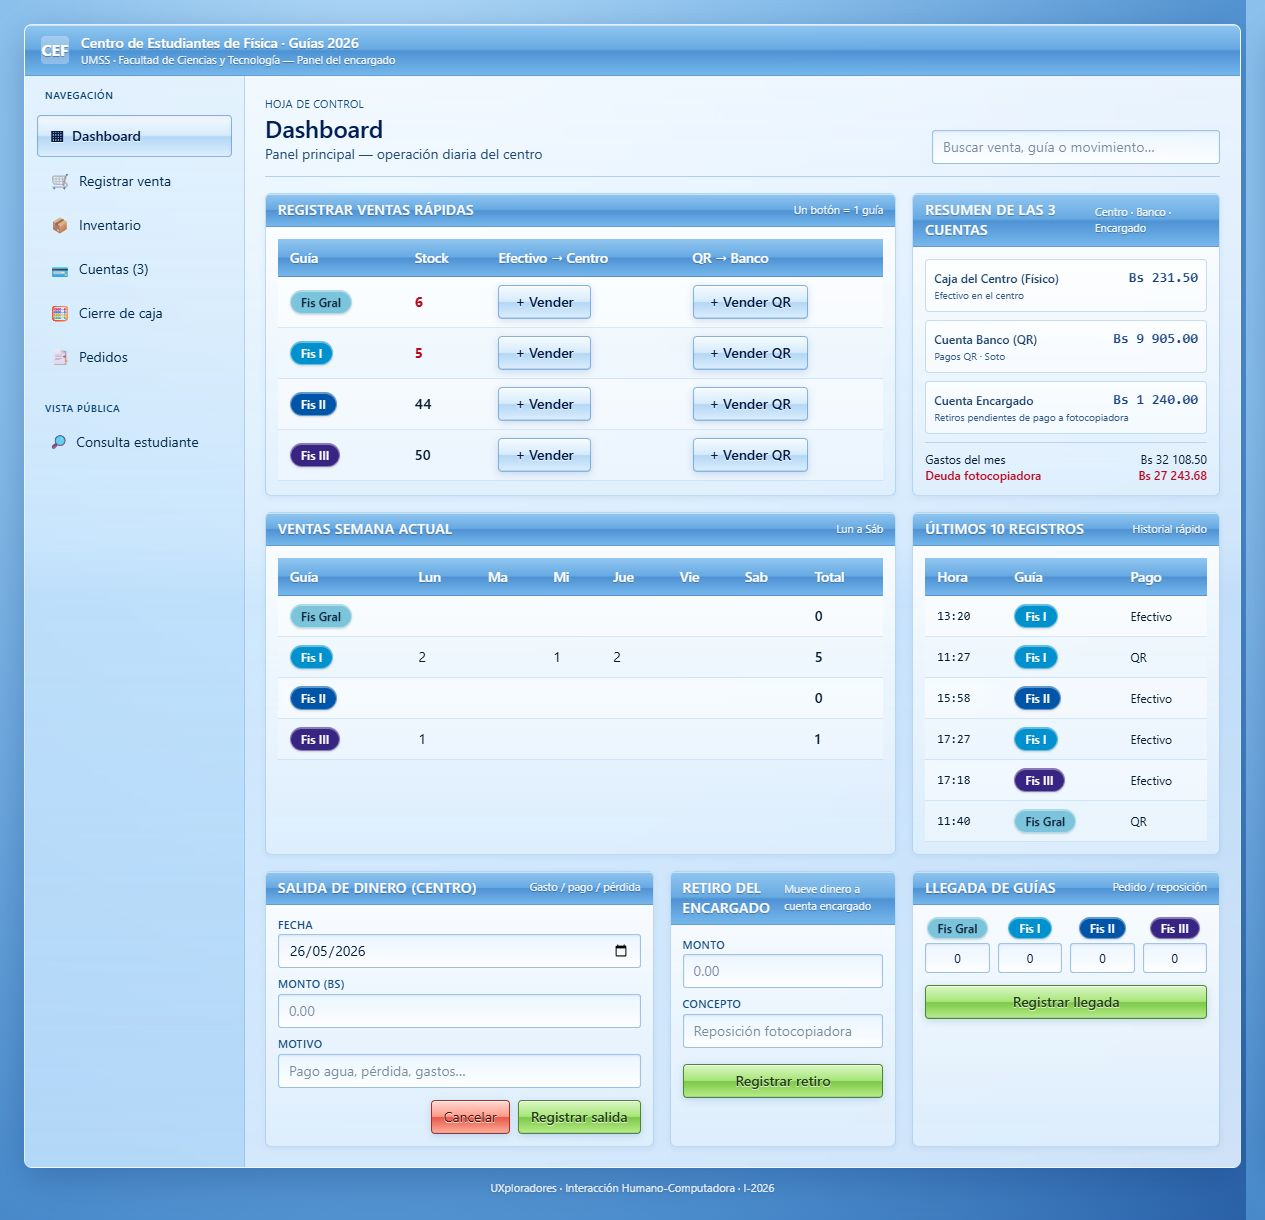
\includegraphics[width=\textwidth,height=0.34\textheight,keepaspectratio]{prototipo_dashboard.png}\\[4pt]
        {\small\textbf{Dashboard}}
    \end{minipage}
    
    \vspace{14pt}
    \begin{minipage}{0.94\textwidth}
        \centering
        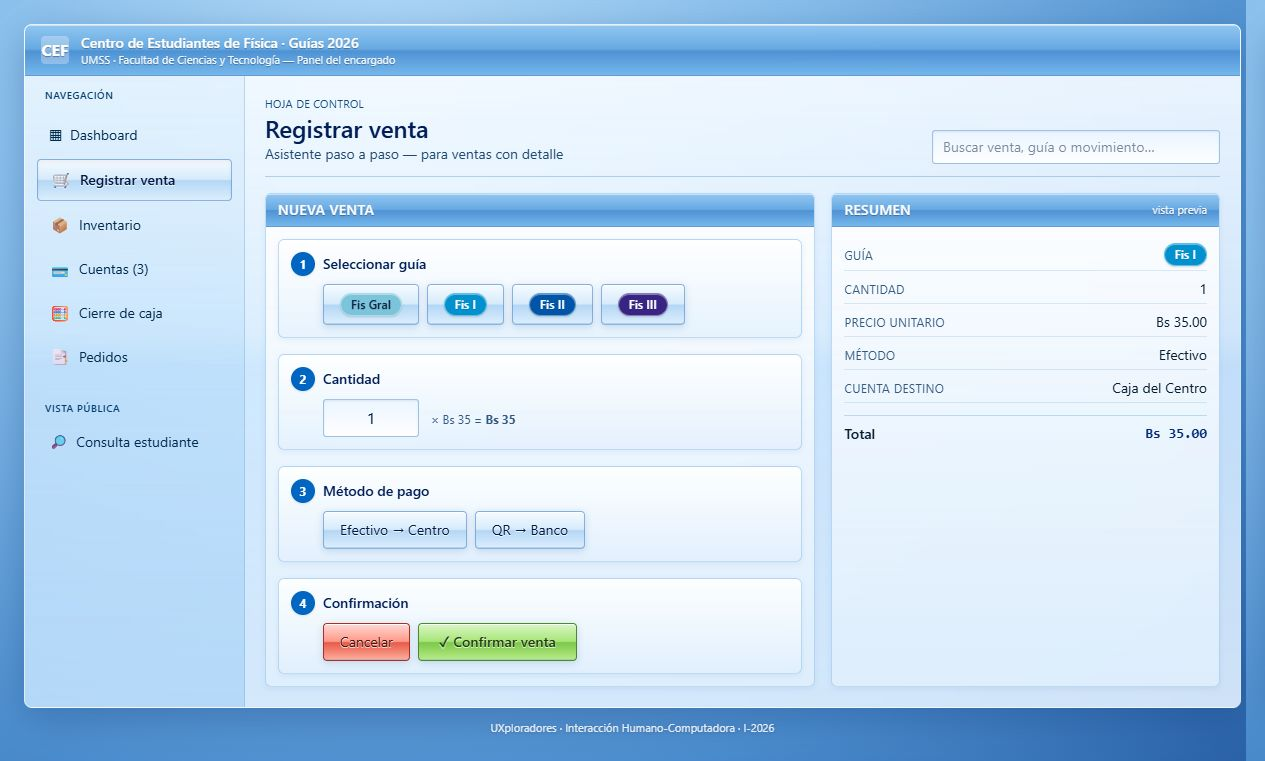
\includegraphics[width=\textwidth,height=0.34\textheight,keepaspectratio]{prototipo_venta.png}\\[4pt]
        {\small\textbf{Registrar entrega}}
    \end{minipage}

    \vspace{8pt}
    \captionof{figure}{Pantallas de acceso principal y registro de entrega.}
\end{center}

\clearpage

\begin{center}
    \begin{minipage}{0.88\textwidth}
        \centering
        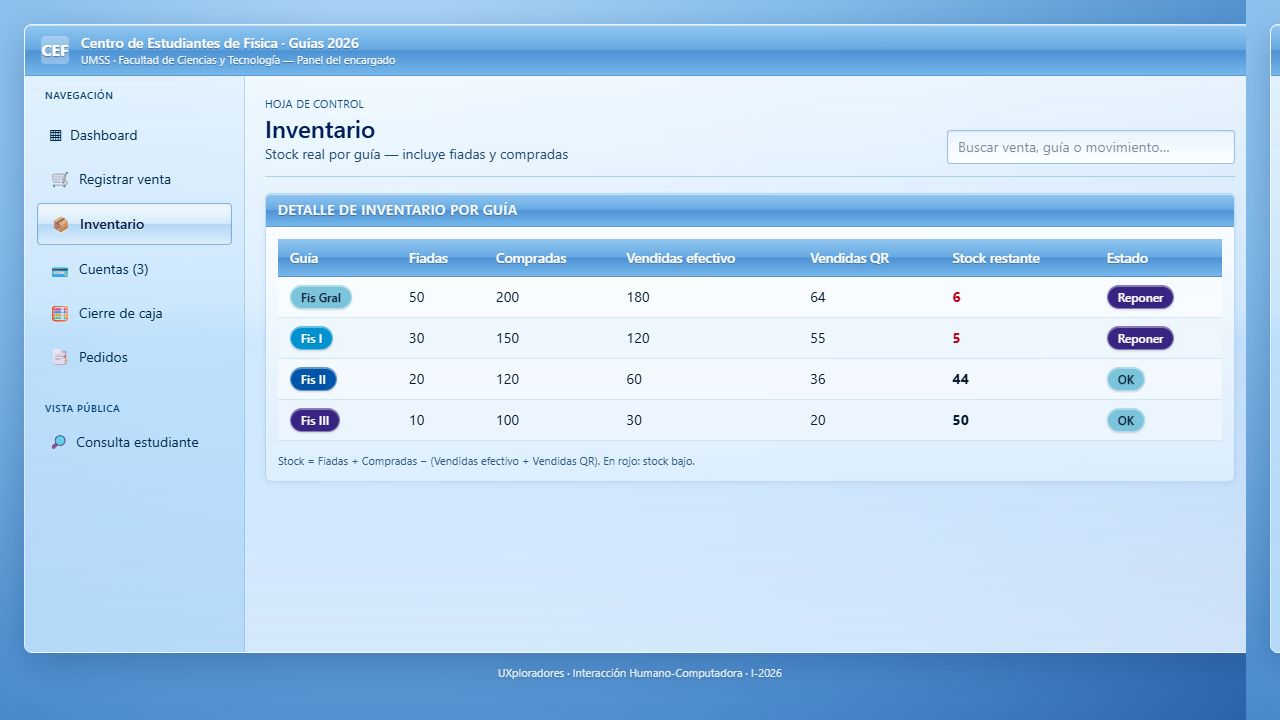
\includegraphics[width=\textwidth,height=0.29\textheight,keepaspectratio]{prototipo_inventario.png}\\[3pt]
        {\small\textbf{Inventario}}
    \end{minipage}
    
    \vspace{12pt}
    \begin{minipage}{0.88\textwidth}
        \centering
        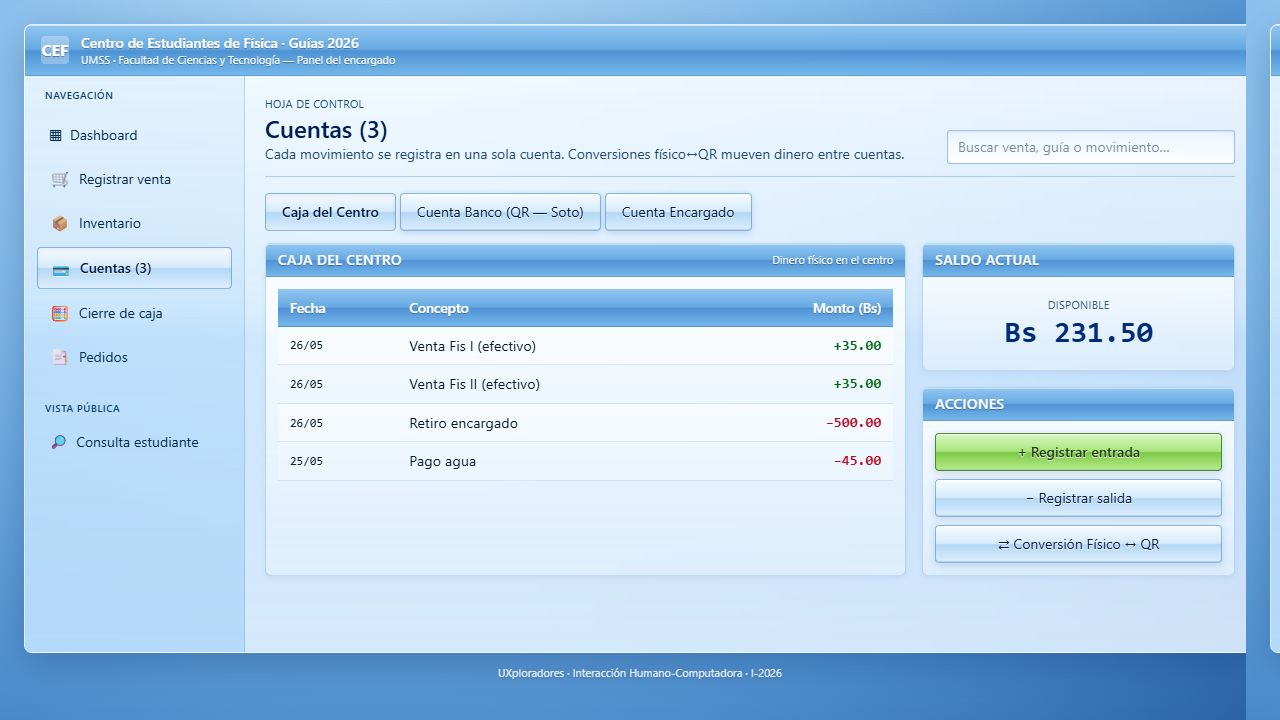
\includegraphics[width=\textwidth,height=0.29\textheight,keepaspectratio]{prototipo_cuentas.png}\\[3pt]
        {\small\textbf{Cuentas}}
    \end{minipage}
    
    \vspace{5pt}
    \captionof{figure}{Pantallas de control de inventario y dinero.}
\end{center}

\clearpage

\begin{center}
    \begin{minipage}{0.88\textwidth}
        \centering
        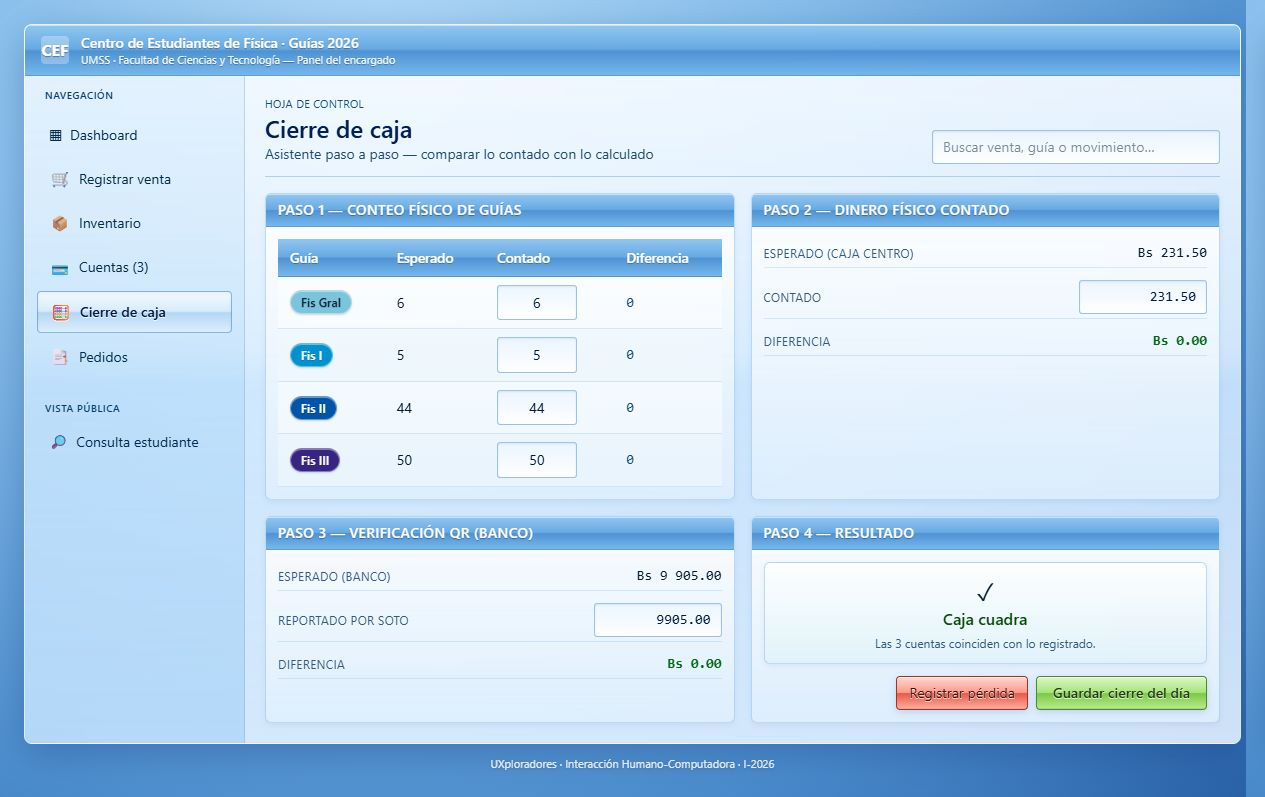
\includegraphics[width=\textwidth,height=0.29\textheight,keepaspectratio]{prototipo_cierre.png}\\[3pt]
        {\small\textbf{Cierre de caja}}
    \end{minipage}
    
    \vspace{12pt}
    \begin{minipage}{0.88\textwidth}
        \centering
        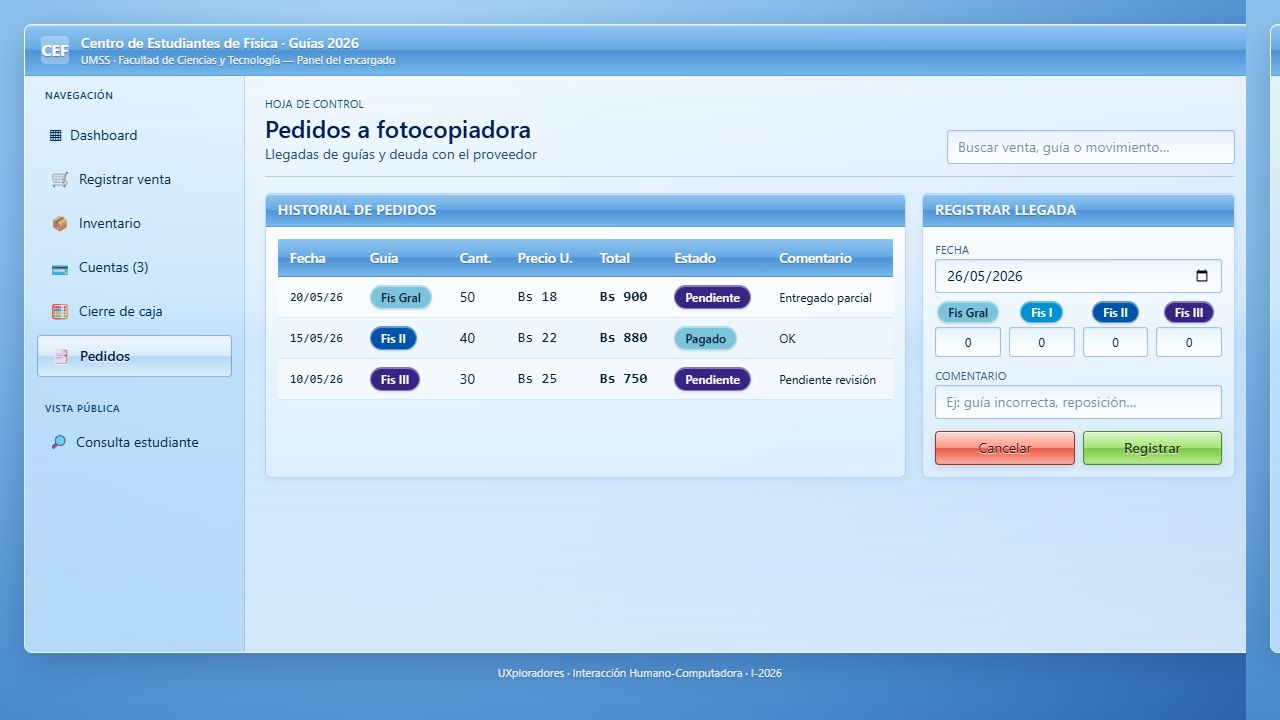
\includegraphics[width=\textwidth,height=0.29\textheight,keepaspectratio]{prototipo_pedidos.png}\\[3pt]
        {\small\textbf{Pedidos}}
    \end{minipage}
    
    \vspace{5pt}
    \captionof{figure}{Pantallas de cierre y reposicion de guias.}
\end{center}

\clearpage

\begin{center}
    \begin{minipage}{0.86\textwidth}
        \centering
        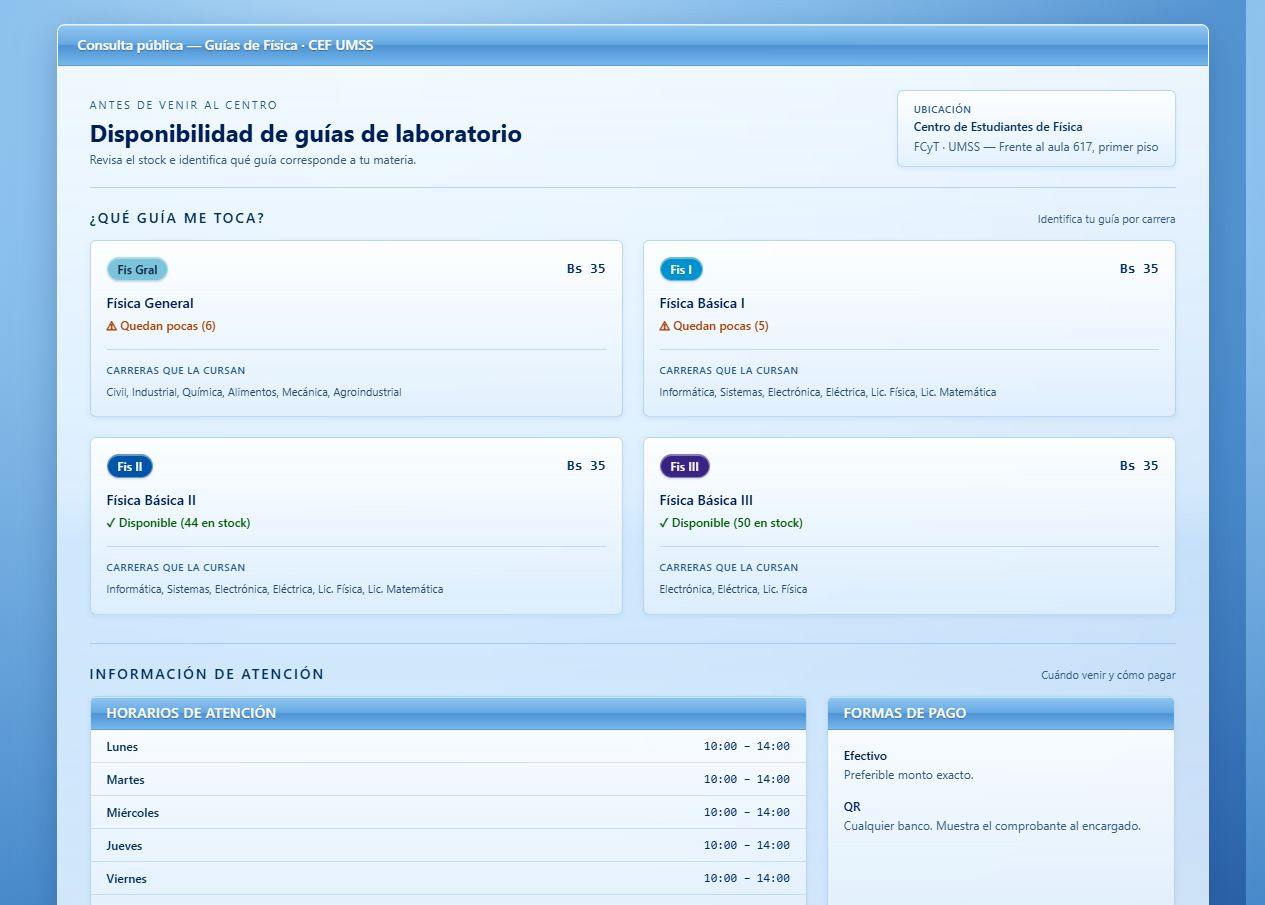
\includegraphics[width=\textwidth,height=0.31\textheight,keepaspectratio]{prototipo_consulta.png}\\[3pt]
        {\small\textbf{Consulta estudiante}}
    \end{minipage}
    
    \vspace{5pt}
    \captionof{figure}{Pantalla publica para estudiantes compradores.}
\end{center}

\FloatBarrier

\section{Prueba de usabilidad}

La prueba de usabilidad se realizo de forma remota con usuarios representativos de los dos perfiles principales del proyecto: encargados del Centro de Estudiantes y estudiantes compradores. El objetivo fue observar si las tareas principales podian completarse sin explicacion extensa, identificando dificultades de navegacion, comprension de informacion y registro de datos.

\begin{center}
\small
\begin{tabularx}{\textwidth}{|B{1.7cm}|B{2.8cm}|Y|B{2.6cm}|}
\hline
Usuario & Perfil & Tareas evaluadas & Resultado \\
\hline
E1 & Encargado & Identificar stock bajo, registrar entrega QR, revisar inventario, revisar cuentas y cierre de caja. & Completo, pero encontro bugs en venta, cuentas y cierre. \\
\hline
E2 & Encargado & Identificar stock bajo, registrar entrega QR, revisar inventario, revisar cuentas y cierre de caja. & Completo, pero encontro confusion en letras, cuentas y cierre. \\
\hline
C1 & Estudiante comprador & Consultar guia de Fisica II, stock, precio, ubicacion y forma de pago. & Completo sin ayuda. \\
\hline
\end{tabularx}
\end{center}

\subsection{Resultados por tarea}

\begin{center}
\small
\begin{tabularx}{\textwidth}{|B{3.3cm}|Y|B{2.4cm}|}
\hline
Tarea & Observacion & Resultado \\
\hline
Consulta estudiante & El estudiante comprador encontro la guia de Fisica II, verifico stock, precio, ubicacion y forma de pago. Indico que la informacion le permite decidir si debe ir al Centro de Estudiantes. & Sin problema \\
\hline
Dashboard / stock bajo & Ambos encargados identificaron rapidamente las guias con stock bajo. E1 lo hizo en aproximadamente 8 segundos. E2 encontro rapido la informacion, pero menciono confusion con las letras usadas para diferenciar las guias. & Completo con observacion \\
\hline
Registrar entrega QR & Ambos encargados pudieron registrar una entrega con pago QR. E1 detecto un bug o dificultad al ver el stock actual: la informacion existe, pero no se nota a simple vista y depende demasiado del panel lateral. E2 no encontro problema en esta tarea. & Completo con bug visual \\
\hline
\end{tabularx}
\end{center}

\vspace{6pt}

\begin{center}
\small
\begin{tabularx}{\textwidth}{|B{3.3cm}|Y|B{2.4cm}|}
\hline
Tarea & Observacion & Resultado \\
\hline
Inventario & Ambos encargados verificaron que el inventario se actualiza correctamente despues de registrar la entrega. No se detecto problema visual importante en esta pantalla. & Sin problema \\
\hline
Cuentas & E1 observo que el dinero no se actualiza automaticamente y que las fechas resultan confusas. E2 indico que el registro de dinero deberia ser automatico y que la seccion de acciones rapidas no es clara. & Problema alto \\
\hline
Cierre de caja & E1 encontro un bug porque el cierre no actualiza el dinero y sugirio registrar el nombre del encargado. E2 considero que los pasos siguen siendo confusos y observo problemas con los botones finales. Ambos evidencian que falta historial de cierres o errores. & Problema alto \\
\hline
\end{tabularx}
\end{center}

\vspace{6pt}

\section{Evaluacion heuristica}

Tambien se realizo una revision rapida del prototipo con criterios de usabilidad. Se priorizaron aspectos visibles durante el uso del sistema.

\begin{center}
\small
\begin{tabularx}{\textwidth}{|B{3.4cm}|Y|B{2.1cm}|}
\hline
Criterio & Observacion & Severidad \\
\hline
Visibilidad del estado & El sistema muestra estados de carga, error o confirmacion en las pantallas principales. & Baja \\
\hline
Prevencion de errores & Algunas acciones validan cantidad, stock y montos antes de guardar, pero los bugs en Cuentas y Cierre muestran que aun falta controlar mejor la relacion entre movimientos de guias y dinero. & Alta \\
\hline
Consistencia & La navegacion y los paneles mantienen una estructura similar en todo el sistema. & Baja \\
\hline
Reconocimiento antes que memoria & Las guias se muestran con nombre, materia, precio y stock para evitar que el usuario memorice datos. & Baja \\
\hline
Correspondencia con el mundo real & La separacion entre caja del Centro, Banco QR y Encargado ayuda a representar el manejo real del dinero, pero requiere mayor explicacion visual. & Media \\
\hline
Control y libertad del usuario & En el cierre de caja no queda suficientemente claro que hacer cuando se detecta una diferencia o cuando los botones finales no funcionan como espera el encargado. & Alta \\
\hline
\end{tabularx}
\end{center}

\section{Problemas encontrados y recomendaciones}

Los codigos P-01 a P-07 son identificadores internos de los problemas detectados durante la prueba. Sirven para relacionar cada hallazgo con su severidad y con una recomendacion concreta de mejora.

\begin{center}
\small
\begin{tabularx}{\textwidth}{|B{1.1cm}|Y|B{1.9cm}|Y|}
\hline
Cod. & Problema encontrado & Severidad & Recomendacion \\
\hline
P-01 & En Registrar entrega, E1 pudo completar la venta en 15 segundos, pero percibio un bug al revisar el stock actual. La informacion existe, pero queda poco visible y depende demasiado del panel lateral. & Media & Aumentar jerarquia visual del stock disponible, ubicarlo cerca del boton de confirmacion y mostrar alerta si queda poco stock. \\
\hline
P-02 & En Cuentas, E1 observo que el dinero no se actualiza despues de una entrega. E2 tambien esperaba que el registro de dinero sea automatico. Esto rompe la relacion entre venta, cuenta y cierre. & Alta & Vincular automaticamente las entregas con movimientos de dinero segun metodo de pago: efectivo hacia Caja del Centro y QR hacia Banco. \\
\hline
P-03 & En Cuentas, las fechas y la seccion de acciones rapidas no son suficientemente claras para los encargados. & Media & Mejorar jerarquia visual, agrupar movimientos por cuenta, aclarar fechas y renombrar acciones con verbos mas especificos. \\
\hline
\end{tabularx}
\end{center}

\vspace{6pt}

\begin{center}
\small
\begin{tabularx}{\textwidth}{|B{1.1cm}|Y|B{1.9cm}|Y|}
\hline
Cod. & Problema encontrado & Severidad & Recomendacion \\
\hline
P-04 & En Cierre de caja, E1 observo que el dinero no se actualiza correctamente. E2 indico que los pasos siguen siendo confusos y que los botones finales generan dudas. & Alta & Convertir el cierre en un asistente por pasos, explicar cada accion final y mostrar claramente que se guardo o que falta corregir. \\
\hline
P-05 & Falta historial visible de cierres, errores o problemas detectados durante el cierre de caja. & Alta & Agregar historial de cierres con fecha, diferencias, encargado responsable y observaciones. \\
\hline
\end{tabularx}
\end{center}

\vspace{6pt}

\begin{center}
\small
\begin{tabularx}{\textwidth}{|B{1.1cm}|Y|B{1.9cm}|Y|}
\hline
Cod. & Problema encontrado & Severidad & Recomendacion \\
\hline
P-06 & Un encargado sugirio registrar el nombre del encargado durante el cierre de caja. & Media & Agregar campo ``Encargado responsable'' al registrar cierre y mostrarlo en el historial. \\
\hline
P-07 & En la vista estudiante no se detectaron problemas importantes; el usuario encontro precio, stock, ubicacion y formas de pago. & Baja & Mantener la estructura actual y priorizar solo ajustes visuales menores si fueran necesarios. \\
\hline
\end{tabularx}
\end{center}

\section{Sintesis de la evaluacion}

La evaluacion combino pruebas de usabilidad y revision heuristica. Los encargados realizaron tareas reales del Centro de Estudiantes: identificar stock bajo, registrar una entrega QR, revisar inventario, revisar cuentas y validar el cierre de caja. El estudiante comprador reviso una guia de Fisica II, su stock, precio, ubicacion y forma de pago. La vista publica funciono sin problemas importantes; en cambio, las pantallas administrativas concentraron los errores mas graves: Cuentas no actualiza el dinero automaticamente, Cierre de caja sigue siendo confuso y falta historial visible de cierres o errores.

\begin{center}
\small
\begin{tabularx}{\textwidth}{|B{4.2cm}|Y|}
\hline
Tecnica aplicada & Aporte \\
\hline
Usabilidad con encargados & Detecto bugs en venta, cuentas y cierre de caja. \\
\hline
Usabilidad con estudiante comprador & Confirmo que la vista publica permite encontrar guia, stock, precio, ubicacion y forma de pago sin ayuda. \\
\hline
Evaluacion heuristica & Clasifico problemas por severidad y los convirtio en recomendaciones de mejora. \\
\hline
\end{tabularx}
\end{center}

\clearpage
\section{Conclusion}

El prototipo cumple parcialmente el objetivo de la Semana 4: permite ejecutar y evaluar los flujos principales, pero todavia no puede considerarse una version final. La prueba con el estudiante comprador mostro que la vista publica es suficientemente clara para consultar disponibilidad, precio, ubicacion y forma de pago. Esto indica que la informacion orientada al comprador esta bien organizada y permite decidir si vale la pena ir al Centro de Estudiantes.

En cambio, las pruebas con encargados evidenciaron que el flujo administrativo requiere correcciones importantes. El registro de entrega pudo completarse, pero el stock actual no siempre se percibe de forma clara. Inventario funciono correctamente, pero Cuentas y Cierre de caja concentraron los problemas de mayor severidad: el dinero no se actualiza automaticamente despues de registrar entregas, las fechas y acciones rapidas generan confusion, los pasos finales del cierre no son suficientemente claros y falta un historial visible de cierres, diferencias o errores.

Por tanto, la siguiente iteracion debe priorizar la automatizacion entre entregas, cuentas y cierre de caja; mejorar la jerarquia visual del stock y de los saldos; registrar al encargado responsable durante el cierre; y agregar un historial que permita revisar cierres anteriores. Con estas correcciones, el prototipo podria pasar de una version funcional inicial a una version mas estable y comprensible para el uso real del Centro de Estudiantes.

\end{document}
